\documentclass[12pt,border=1pt]{standalone}
\usepackage[T1]{fontenc}
\IfFileExists{newtxtext.sty}{\usepackage{newtxtext,newtxmath}}{\usepackage{mathptmx}}
\usepackage{amsmath,amssymb}
\usepackage[table]{xcolor}
\usepackage{tikz}
\usetikzlibrary{arrows.meta,positioning,fit,calc,decorations.pathreplacing}
\tikzset{blk/.style={draw=black!55,rounded corners=2pt,align=center,font=\footnotesize,inner sep=4pt,minimum height=1.05cm},
         nn/.style={blk,fill=orange!12,draw=orange!70!black},
         lat/.style={blk,fill=blue!8,draw=blue!60!black},
         io/.style={blk,fill=black!3},
         arr/.style={-{Stealth[length=2.2mm]},thick,draw=black!65}}
\definecolor{capblue}{RGB}{47,84,150}
\definecolor{linkblue}{RGB}{17,85,204}
\definecolor{ganttA}{RGB}{11,90,110}
\definecolor{ganttB}{RGB}{20,150,160}
\definecolor{rowhl}{RGB}{253,236,224}
\definecolor{rowhl2}{RGB}{224,244,238}
\begin{document}
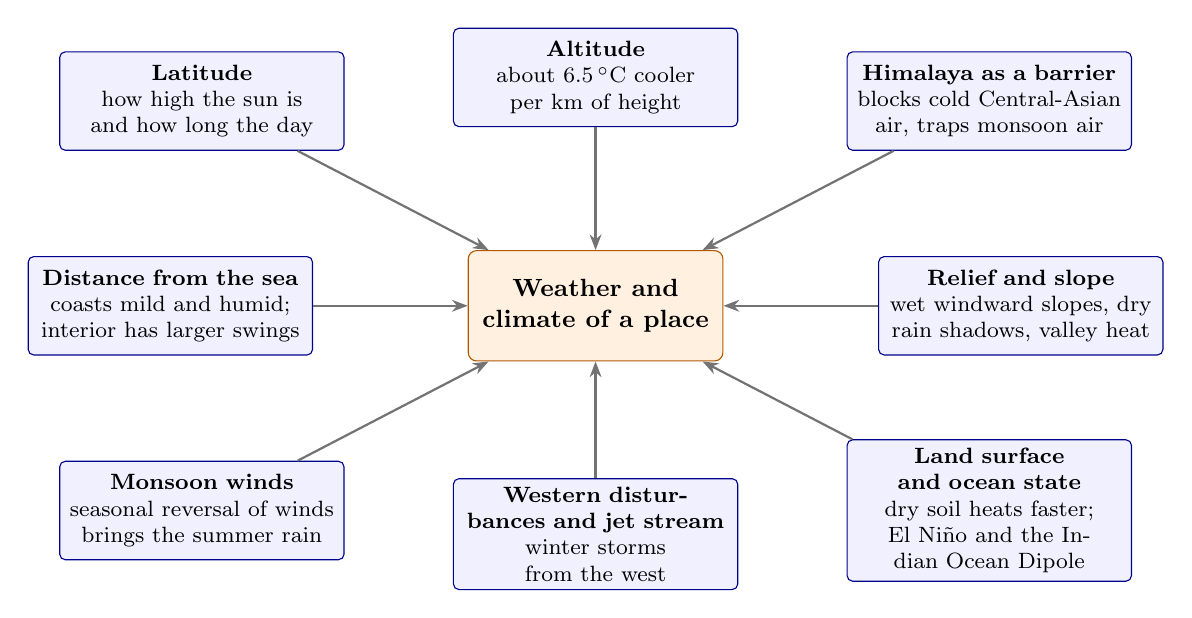
\begin{tikzpicture}[
  fac/.style={draw=blue!55!black,fill=blue!6,rounded corners=2pt,text width=3.4cm,align=center,font=\footnotesize,minimum height=1.25cm,inner sep=3pt},
  mid/.style={draw=orange!70!black,fill=orange!12,rounded corners=3pt,text width=3.0cm,align=center,font=\small\bfseries,minimum height=1.4cm},
  ar2/.style={-{Stealth[length=2mm]},thick,black!55}]
\node[mid] (c) at (0,0) {Weather and climate of a place};
\node[fac] (f1) at (-5.0, 2.6) {\textbf{Latitude}\\ how high the sun is and how long the day};
\node[fac] (f2) at (0, 2.9) {\textbf{Altitude}\\ about 6.5\,$^\circ$C cooler per km of height};
\node[fac] (f3) at (5.0, 2.6) {\textbf{Himalaya as a barrier}\\ blocks cold Central-Asian air, traps monsoon air};
\node[fac] (f4) at (-5.4, 0) {\textbf{Distance from the sea}\\ coasts mild and humid; interior has larger swings};
\node[fac] (f5) at (5.4, 0) {\textbf{Relief and slope}\\ wet windward slopes, dry rain shadows, valley heat};
\node[fac] (f6) at (-5.0,-2.6) {\textbf{Monsoon winds}\\ seasonal reversal of winds brings the summer rain};
\node[fac] (f7) at (0,-2.9) {\textbf{Western disturbances and jet stream}\\ winter storms from the west};
\node[fac] (f8) at (5.0,-2.6) {\textbf{Land surface and ocean state}\\ dry soil heats faster; El Ni\~no and the Indian Ocean Dipole};
\foreach \f in {f1,f2,f3,f4,f5,f6,f7,f8} \draw[ar2] (\f) -- (c);
\end{tikzpicture}
\end{document}
